\documentclass[12pt,a4paper]{article}

\usepackage[T1]{fontenc}
\usepackage[brazilian]{babel}
\usepackage{lmodern}
\usepackage[margin=2.5cm]{geometry}
\usepackage{amsmath}
\usepackage{amssymb}
\usepackage{graphicx}
\usepackage{booktabs}
\usepackage{microtype}
\usepackage{natbib}
\usepackage[hidelinks]{hyperref}

\title{Relatório Variável \textit{Wind}}
\author{Allex D'Ávila Brandão}
\date{\today}

\begin{document}

\maketitle

\section{Introdução}
Os dados tem origem do arquivo \texttt{airquality}. O conjunto de dados possui um total de 153 observações. A variável analisada é a Wind, nas observações não foram encontrados nenhum valor \texttt{NA}.

\section{Análise Mensal}
Conforme apresentado na Tabela~\ref{tab:resumo}, as médias mensais de wind, foram calculadas com os meses de maio e setembro. A média geral calculada pelo script segue conforme a Equação~\eqref{eq:media}:

\begin{equation}
\label{eq:media}
\bar{X}_m = \frac{\sum_{i=1}^{n_m} X_{im}}{n_m}
\end{equation}

Na Equação~\eqref{eq:media}, o denominador $n_m$ representa o número de dias efetivamente medidos no mês $m$.

\begin{table}[htbp]
\centering
\caption{Resumo da velocidade do vento (\textit{Wind}) por mês.}
\label{tab:resumo}
\begin{tabular}{ccc}
\toprule
Mês & Média (mph) & Dias Medidos \\
\midrule
5 & 11.62 & 31/31 \\
6 & 10.27 & 30/30 \\
7 & 8.94  & 31/31 \\
8 & 8.79  & 31/31 \\
9 & 10.18 & 30/30 \\
\bottomrule
\end{tabular}
\end{table}

O gráfico da variável ao longo dos meses pode ser visualizada na Figura~\ref{fig:wind}. A análise foi conduzida no ambiente computacional R \citep{rproject} e documentada conforme as boas práticas do ecossistema \citep{xie2018}.

\begin{figure}[htbp]
\centering
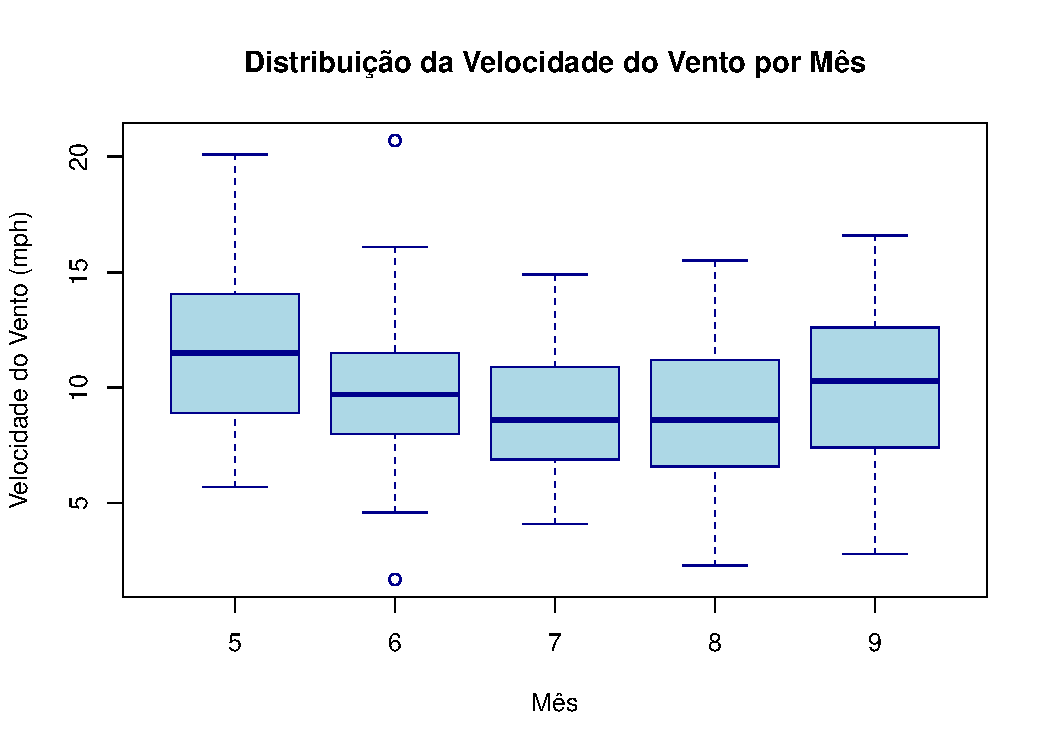
\includegraphics[width=0.7\textwidth]{figura.pdf}
\caption{Distribuição da variável wind}
\label{fig:wind}
\end{figure}

\section*{Declaração de uso de IA}
Foi utilizado o Gemini para ajudar na correção de erros no terminal, comandos Git e estrutura inicial dos blocos do código \LaTeX{}. Todos os arquivos e compilações foram revisados e testados manualmente.

\bibliographystyle{plainnat}
\bibliography{referencias}

\end{document}
